\documentclass[aspectratio=169]{../latex_main/tntbeamer}  % you can pass all options of the beamer class, e.g., 'handout' or 'aspectratio=43'
\usepackage{dsfont}
\usepackage{bm}
\usepackage[english]{babel}
\usepackage[T1]{fontenc}
%\usepackage[utf8]{inputenc}
\usepackage{graphicx}
\graphicspath{ {./figures/} }
\usepackage{algorithm}
\usepackage[ruled,vlined,algo2e,linesnumbered]{algorithm2e}
\usepackage{hyperref}
\usepackage{booktabs}
\usepackage{mathtools}

\usepackage{amsmath,amssymb}

\DeclareMathOperator*{\argmax}{arg\,max}
\DeclareMathOperator*{\argmin}{arg\,min}

\usepackage{amsbsy}
\newcommand{\vect}[1]{\bm{#1}}
%\newcommand{\vect}[1]{\boldsymbol{#1}}

\usepackage{pgfplots}
\pgfplotsset{compat=1.16}
\usepackage{tikz}
\usetikzlibrary{trees} 
\usetikzlibrary{shapes.geometric}
\usetikzlibrary{positioning,shapes,shadows,arrows,calc,mindmap}
\usetikzlibrary{positioning,fadings,through}
\usetikzlibrary{decorations.pathreplacing}
\usetikzlibrary{intersections}
\pgfdeclarelayer{background}
\pgfdeclarelayer{foreground}
\pgfsetlayers{background,main,foreground}
\tikzstyle{activity}=[rectangle, draw=black, rounded corners, text centered, text width=8em]
\tikzstyle{data}=[rectangle, draw=black, text centered, text width=8em]
\tikzstyle{myarrow}=[->, thick, draw=black]

% Define the layers to draw the diagram
\pgfdeclarelayer{background}
\pgfdeclarelayer{foreground}
\pgfsetlayers{background,main,foreground}

% Requires XeLaTeX or LuaLaTeX
%\usepackage{unicode-math}

\usepackage{fontspec}
%\setsansfont{Arial}
\setsansfont{RotisSansSerifStd}[ 
Path=../latex_main/fonts/,
Extension = .otf,
UprightFont = *-Regular,  % or *-Light
BoldFont = *-ExtraBold,  % or *-Bold
ItalicFont = *-Italic
]
\setmonofont{Cascadia Mono}[
Scale=0.8
]

% scale factor adapted; mathrm font added (Benjamin Spitschan @TNT, 2021-06-01)
%\setmathfont[Scale=1.05]{Libertinus Math}
%\setmathrm[Scale=1.05]{Libertinus Math}

% other available math fonts are (not exhaustive)
% Latin Modern Math
% XITS Math
% Libertinus Math
% Asana Math
% Fira Math
% TeX Gyre Pagella Math
% TeX Gyre Bonum Math
% TeX Gyre Schola Math
% TeX Gyre Termes Math

% Literature References
\newcommand{\lit}[2]{\href{#2}{\footnotesize\color{black!60}[#1]}}

%%% Beamer Customization
%----------------------------------------------------------------------
% (Don't) Show sections in frame header. Options: 'sections', 'sections light', empty
\setbeamertemplate{headline}{empty}

% Add header logo for normal frames
\setheaderimage{
	% 
\includegraphics[height=\logoheight]{figures/TNT_darkv4.pdf}
	
\includegraphics[height=\logoheight]{../latex_main/figures/luh_logo_rgb_0_80_155.pdf}
	% 
\includegraphics[height=\logoheight]{figures/logo_tntluh.pdf}
}

% Header logo for title page
\settitleheaderimage{
	% 
\includegraphics[height=\logoheight]{figures/TNT_darkv4.pdf}
	
\includegraphics[height=\logoheight]{../latex_main/figures/luh_logo_rgb_0_80_155.pdf}
	% 
\includegraphics[height=\logoheight]{figures/logo_tntluh.pdf}
}

% Title page: tntdefault 
\setbeamertemplate{title page}[tntdefault]  % or luhstyle
% Add optional title image here
%\addtitlepageimagedefault{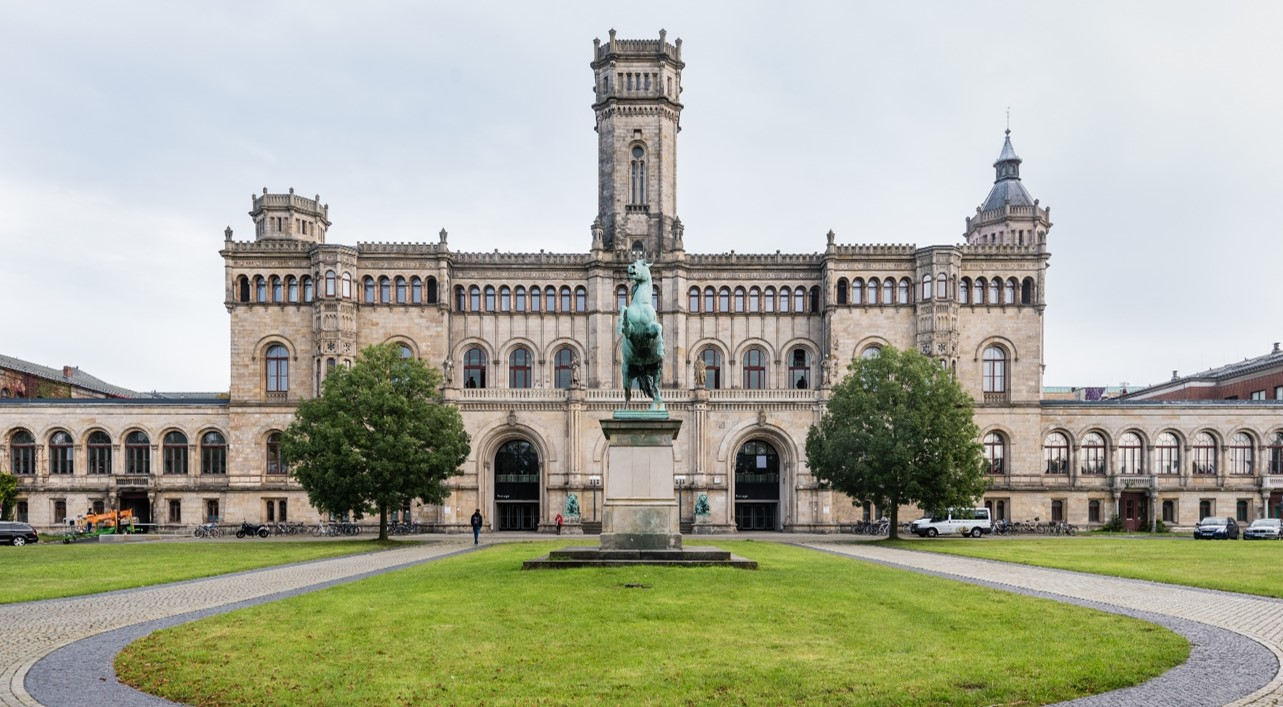
\includegraphics[width=0.65\textwidth]{figures/luh_default_presentation_title_image.jpg}}

% Title page: luhstyle
% \setbeamertemplate{title page}[luhstyle]
% % Add optional title image here
% \addtitlepageimage{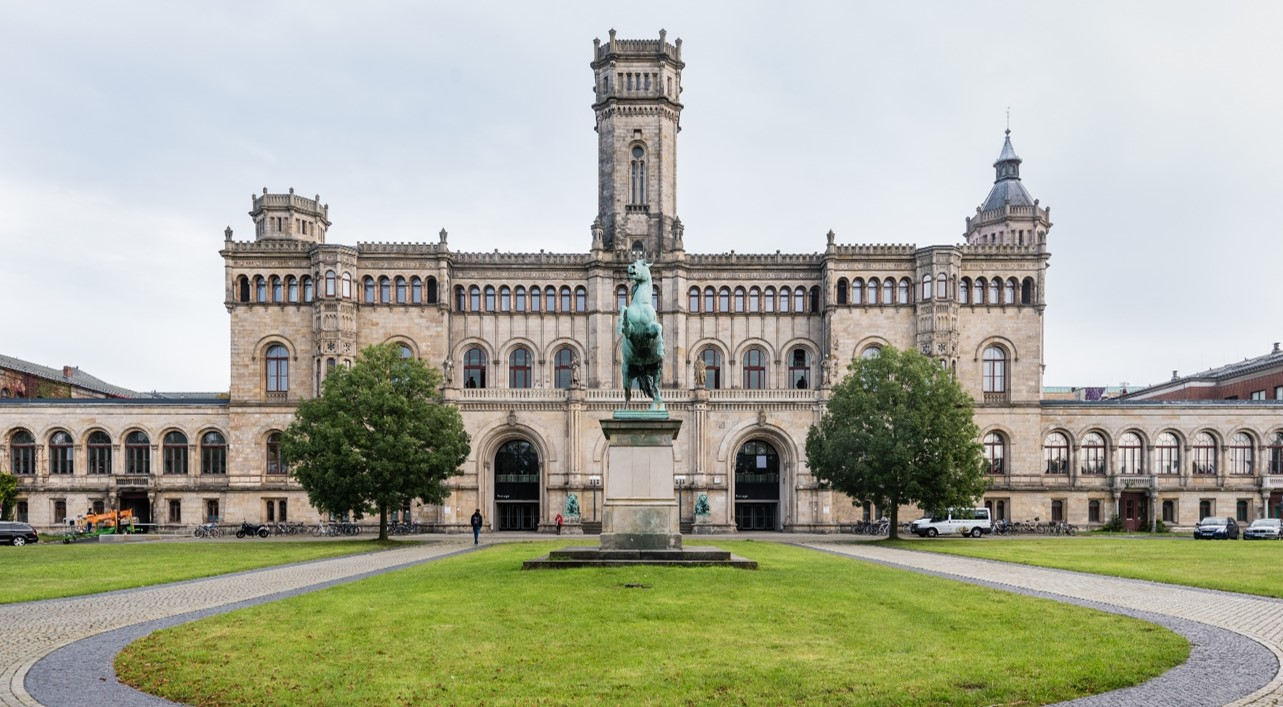
\includegraphics[width=0.75\textwidth]{figures/luh_default_presentation_title_image.jpg}}

\author[Abedjan \& Lindauer]{Ziawasch Abedjan \& Marius Lindauer\\[1em]
	
\includegraphics[height=\logoheight]{../latex_main/figures/luh_logo_rgb_0_80_155.pdf}\qquad
	
\includegraphics[height=\logoheight]{../latex_main/figures/DBIS_Kurzlogo.png}\qquad

\includegraphics[height=\logoheight]{../latex_main/figures/TNT_darkv4}\qquad

\includegraphics[height=\logoheight]{../latex_main/figures/L3S.jpg}	}
\date{Summer Term 2022; \hspace{0.5em} {
\includegraphics[height=1.5em]{../latex_main/figures/Cc-by-nc-sa_icon.svg.png}}; based on \href{https://ds100.org/fa21/}{[DS100]}
}


%%% Custom Packages
%----------------------------------------------------------------------
% Create dummy content
\usepackage{blindtext}

% Adds a frame with the current page layout. Just call \layout inside of a frame.
\usepackage{layout}


%%% Macros
%\renewcommand{\vec}[1]{\mathbf{#1}}
% \usepackage{bm}
%\let\vecb\bm

\title[Introduction]{DS: Data Sampling and Probability}
\subtitle{Extra: permutations and combinations}

\graphicspath{ {./figure/} }
%\institute{}


\begin{document}
	
	\maketitle
	
	
	\begin{frame}{Disclaimer}
	    \begin{itemize}
	        \item This is not a class on probability or combinatorics. 
	        \begin{itemize}
	            \item In other words, this is not Stat 140 or CS 70.
	        \end{itemize}
	        \item This content on its own is not in scope.
	        \begin{itemize}
	            \item In other words, you will never be asked questions like “how many permutations of MISSISSIPPI are there”.
	            \item Instead, we present it in order to (re)explain where the binomial coefficient comes from.
	        \end{itemize}
	        \item This is purely meant to serve as a refresher, and is for your understanding only
	        \item Also, the video will walk through this material in perhaps a more natural fashion.
	    \end{itemize}
	\end{frame}
	
	\begin{frame}{Permutations}
	    Suppose I have five people, boringly named A, B, C, D, and E. In how many ways can I arrange them in a line?
	    \begin{itemize}
	        \item There are 5 options for who can end up first in line (anyone could).
	        \item Given that, there are 4 options for who can end up second in line.
	        \begin{itemize}
	            \item Could be anyone, other than whoever was first (5 - 1 = 4).
	        \end{itemize}
	        \item Given that, there are 3 options for who can end up third in line, and so on.
	    \end{itemize}
	    	       
	       Think of each blank as a position in line, and the number in the blank as the number of people that could end up there.\\
	       
	       \_\_5\_\_ \hspace{2cm}		\_\_4\_\_ \hspace{2cm}		\_\_3\_\_ \hspace{2cm}		\_\_2\_\_	 \hspace{2cm}	\_\_1\_\_

        The result is 5 * 4 * 3 * 2 * 1 = 120, which we denote as 5! (read “five factorial”). In general,\\
        \hspace{4cm} n! = n * (n - 1) * (n - 2) * … * 3 * 2 * 1


	\end{frame}
	
	\begin{frame}{Permutations}
	    How many ways can I arrange 3 of {A, B, C, D, E} in a line?

	    \begin{itemize}
	        \item 5 options for who is first.
	        \item 4 options for who is second.
	        \item 3 options for who is third.
	        \item Nobody after these three.
	    \end{itemize}

	      \hspace{4cm} \_\_5\_\_ \hspace{2cm}		\_\_4\_\_ \hspace{2cm}		\_\_3\_\_ 

       This result is 5 * 4 * 3 = 60. Note, we can also write 5 * 4 * 3 as\\
        \begin{align*}
            5 * 4 * 3 &= (5 * 4 * 3 * 2 * 1) / (2 * 1) \\
            &= 5! / 2! = 5! / (5 - 3)!
        \end{align*}
    What are the implications of this?
	\end{frame}
	
	
	\begin{frame}{Permutations}
	    In general: if I have n objects, and want to select k of them in a way that order matters, then the number of ways I can do this is

	    \begin{equation*}
	        \frac{n!}{(n-k)!}
	    \end{equation*}
        Again: this is not a class that covers counting!
        \begin{itemize}
            \item This result, by itself, will (almost certainly) never appear again in this class
            \item It’s more here to serve as an intermediate step in what comes next.
        \end{itemize}

	\end{frame}
	
		\begin{frame}{Combinations}
	    Now, suppose I want to select three people from {A, B, C, D, E}, but in a way that order does not matter.

        \begin{itemize}
            \item If order mattered, ABE, EAB, BAE, etc. would count as different arrangements.
            \item But if order does not matter, then the above three arrangements are all the same – they contain the same 3 people!
            \item If order does not matter, there are fewer ways to make our selections. 
        \end{itemize}
        How can we use our previous answer to help us here?
        \begin{itemize}
            \item How many times did we overcount?
            \item Each unique group of three people is counted 3! = 6 times.
            \begin{itemize}
                \item ABE, AEB, BAE, BEA, EAB, EBA are really all the same now.
                \item We need to divide our previous answer by the number of times we overcounted!
            \end{itemize}
        \end{itemize}

	\end{frame}
	
	
	\begin{frame}{Combinations}
	    Dividing our previous answer by 3! yields


        \begin{equation*}
            \frac{\frac{5!}{2!}}{3!} = \frac{5!}{2!3!}
        \end{equation*}
        This quantity is the number of ways we can select 3 objects from a set of 5, in a way that order does not matter.\\
        
        More generally, the number of ways we can select k objects from a set of n, in a way that order does not matter (and where k, n are both non-negative integers, and k \leq n) is:

        \begin{equation*}
            \binom{n}{k}= \frac{n!}{(n-k)!k!}
        \end{equation*}
        The symbol on the left is referred to as the binomial coefficient, and is read “n choose k.”

	\end{frame}
	
	
	\begin{frame}{Combinations}
	    Here are some examples on how we can (and will) use the binomial coefficient.
        \begin{itemize}
            \item How many ways can we flip a coin (whose flips are independent of one another) 4 times and see 2 heads?
            \begin{itemize}
                \item Equivalent question: how many different ways can we order the string “HHTT”?
                \item There are 4 “positions.” Choose 2 of them to be H (the remaining 4 will be T).
                \item This is 4 choose 2, or 6. (Enumerated: HHTT, HTHT, HTTH, TTHH, THTH, THHT.)
            \end{itemize}
            \item Suppose we have a bag of marbles that contains marbles, some of which are blue. How many ways can we draw 7 marbles, such that 4 are blue and 3 are not blue?
            \begin{itemize}
                \item We have 7 draws. Choose 4 of them to be blue (the remaining automatically are not).
                \item This is 7 choose 3, or 35 
            \end{itemize}
            \item Note: The above answers (and algebra) imply that $\binom{n}{k}=\binom{n}{n-k}$
            \begin{itemize}
                \item Choosing k successes is equivalent to choosing n - k failures.
            \end{itemize}
        \end{itemize}

	\end{frame}
	
	\begin{frame}{What about order?}
	    \begin{columns}
	        \begin{column}{.4\textwidth}
	            You may be wondering – why did we use the binomial coefficient to determine the number of orderings of 2 heads and 2 tails (HHTT, HTHT, HTTH, TTHH, THTH, THHT), when the whole point was that order doesn’t matter?\\
	            \bigskip
	            The order in which we declare the positions is what doesn’t matter here. The contents of each position, though, do matter. 
	        \end{column}
	        
	        \begin{column}{.5\textwidth}
	           \begin{figure}
	               \centering
	               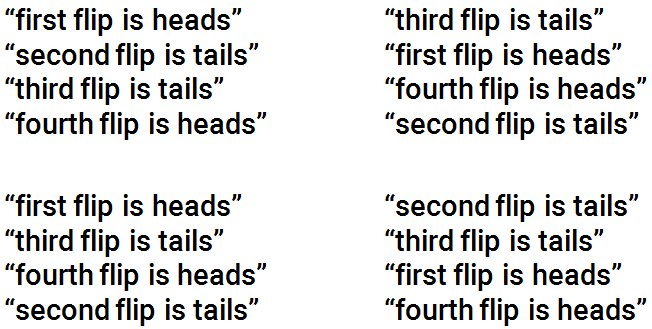
\includegraphics[scale=.3]{Bild15}
	           \end{figure}
	           These are all equivalent! They all equate to the ordering HTTH.\\
	           
	           The order in which you tell me what flip goes where is not of importance. This is why we use choosing here.

	        \end{column}
	        
	    \end{columns}
	    
	\end{frame}
	
	\begin{frame}{Another interpretation}
	    How many ways can we flip a coin (whose flips are independent of one another) 4 times and see 2 heads?
        \begin{itemize}
            \item Equivalent problem to determining the number of rearrangements of HHTT.
            \item Let’s label them uniquely: H1, H2, T1, T2.
            \item There are 4 objects, so there are 4! orders.
            \item But, some of these orderings are really the same!
            \begin{itemize}
                \item “H1 H2 T1 T2” is really the same as “H2 H1 T2 T1” and “H1 H2 T2 T1.”
                \item These should all count as one “ordering.”
                \item There are 2! ways to arrange the two Hs amongst themselves.
                \item There are 2! ways to arrange the two Ts amongst themselves.
            \end{itemize}
            \item Dividing out the repetition yields, as we saw before, $\frac{4!}{2!2!}$
        \end{itemize}

	\end{frame}
	
	\begin{frame}{Extension to multiple categories}
	    How many ways can I select 7 marbles from a bag such that 4 are blue, 2 are green, and 1 is red? (e.g. bgbbbgr, bbbrgbg, brbgbgb, etc.)\\
	    \bigskip
	    Again, there are two interpretations.

        \begin{align*}
            \binom{7}{4}\cdot \binom{3}{2} \cdot \binom{1}{1} \qquad \qquad \frac{7!}{4!2!1!}
        \end{align*}

	\end{frame}
	
	
	\begin{frame}{Extension to multiple categories}
	    How many ways can I select 7 marbles from a bag such that 4 are blue, 2 are green, and 1 is red? (e.g. bgbbbgr, bbbrgbg, brbgbgb, etc.)\\
	    \bigskip
	    Again, there are two interpretations.

        \begin{align*}
            \binom{7}{4}\cdot \binom{3}{2} \cdot \binom{1}{1} \qquad \qquad \frac{7!}{4!2!1!}
        \end{align*}

	\end{frame}
	
	
	\begin{frame}{Extension to multiple categories}
	    How many ways can I select 7 marbles from a bag such that 4 are blue, 2 are green, and 1 is red? (e.g. bgbbbgr, bbbrgbg, brbgbgb, etc.)\\
	    \bigskip
	    Again, there are two interpretations.

        \begin{figure}
                \centering
                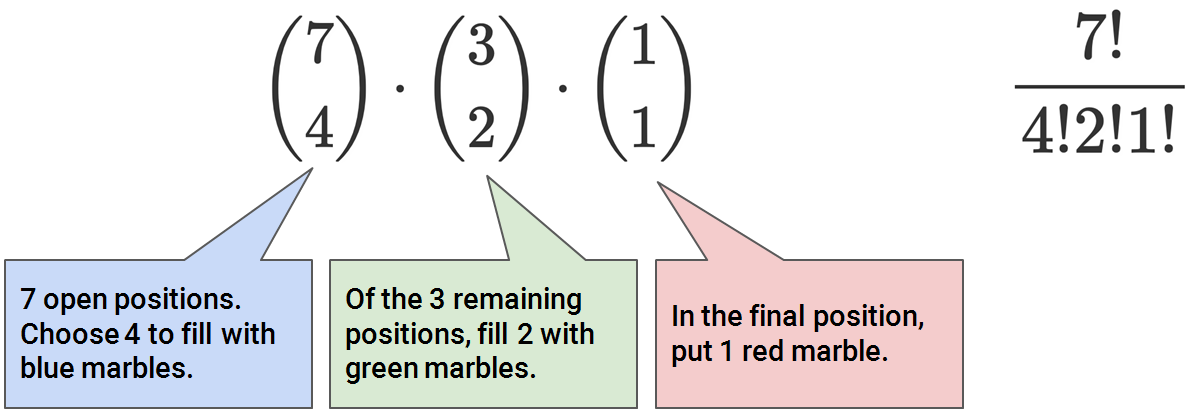
\includegraphics[scale=.4]{Bild16}
            \end{figure}


	\end{frame}
	
	
	
	
	\begin{frame}{Extension to multiple categories}
	    How many ways can I select 7 marbles from a bag such that 4 are blue, 2 are green, and 1 is red? (e.g. bgbbbgr, bbbrgbg, brbgbgb, etc.)\\
	    \bigskip
	    Again, there are two interpretations.
            \begin{figure}
                \centering
                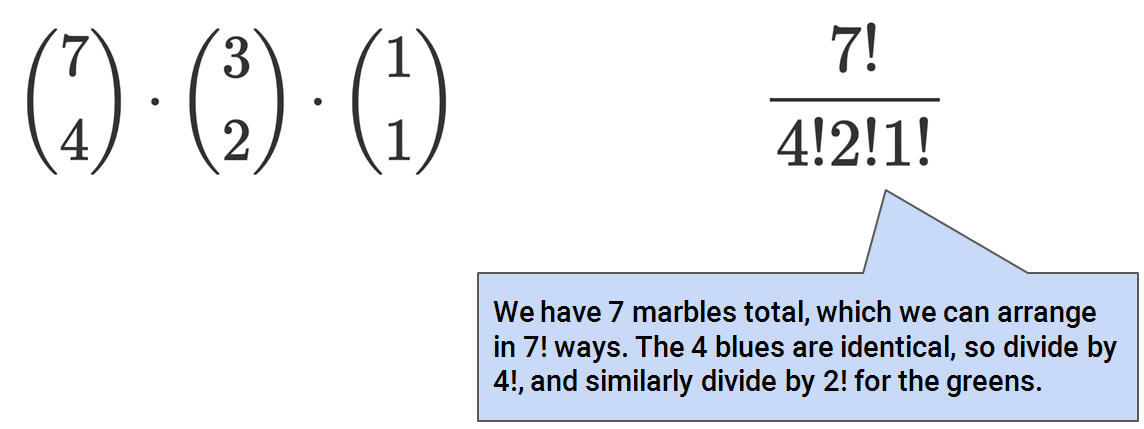
\includegraphics[scale=.4]{Bild17}
            \end{figure}

	\end{frame}
	
	
	
	
	
	\begin{frame}{Extension to multiple categories}
	    How many ways can I select 7 marbles from a bag such that 4 are blue, 2 are green, and 1 is red? (e.g. bgbbbgr, bbbrgbg, brbgbgb, etc.)\\
	    \bigskip
	    Again, there are two interpretations.

        \begin{align*}
            \binom{7}{4}\cdot \binom{3}{2} \cdot \binom{1}{1} \qquad  = \qquad \frac{7!}{4!2!1!}
        \end{align*}
        Unsurprisingly, they are equal!
	\end{frame}
	
	
	
	
	
	
\end{document}